\documentclass[11pt, oneside]{article}
\usepackage[letterpaper, margin=2cm]{geometry}
\usepackage{MATH667}

\begin{document}
\noindent \textbf{\Large{Caleb Logemann \\
MATH667 Hyperbolic Partial Differential Equations \\
Homework 4
}}

%\lstinputlisting[language=MATLAB]{H01_23.m}
Solve Burgers' equation
\begin{gather}
    u_t + \p{\frac{u^2}{2}}_x = 0 \qquad x \in \br{-5, 5} \\
    u(x, 0) = 
    \begin{cases}
      u_l & x \le 0 \\
      u_r & x > 0
    \end{cases}
\end{gather}
with the following Riemann initial data sets.

\begin{enumerate}
  \item[(a)]
    \[
      u(x, 0) =
      \begin{cases}
        1 & x \le 0 \\
        -0.5 & x > 0
      \end{cases}
    \]

  \item[(b)]
    \[
      u(x, 0) =
      \begin{cases}
        -1 & x \le 0 \\
        0.5 & x > 0
      \end{cases}
    \]
\end{enumerate}
\begin{enumerate}
  \item % #1 Done
    Godunov's method uses an exact Riemann solver and is implemented in the
    following function.
    \lstinputlisting[language=MATLAB]{godunov.m}
    The Local Lax-Friedrichs method uses the local maximum wave speed in the
    flux.
    Note that since we are taking the maximum of a linear function, I just took
    the maximum at the endpoints.
    \lstinputlisting[language=MATLAB]{localLaxFriedrichs.m}
    The following script now uses the previous two functions to solve the
    Riemann problems given previously.
    \lstinputlisting[language=MATLAB]{H04.m}
    The following images are produced.
    Both methods give good solutions, however the Godunov method is slightly
    less diffusive than the Local Lax-Friedrichs method.
    \begin{center}
      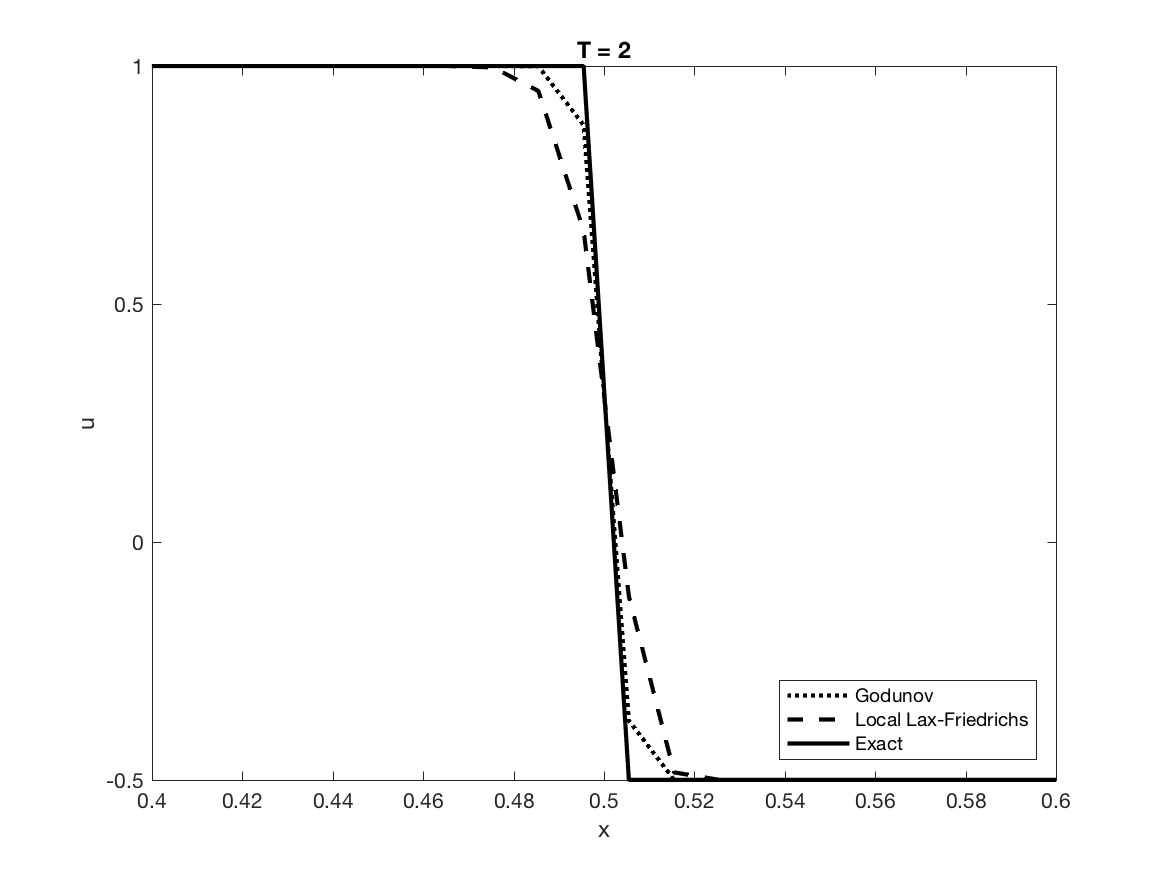
\includegraphics[scale=0.8]{Figures/04_01.png}
      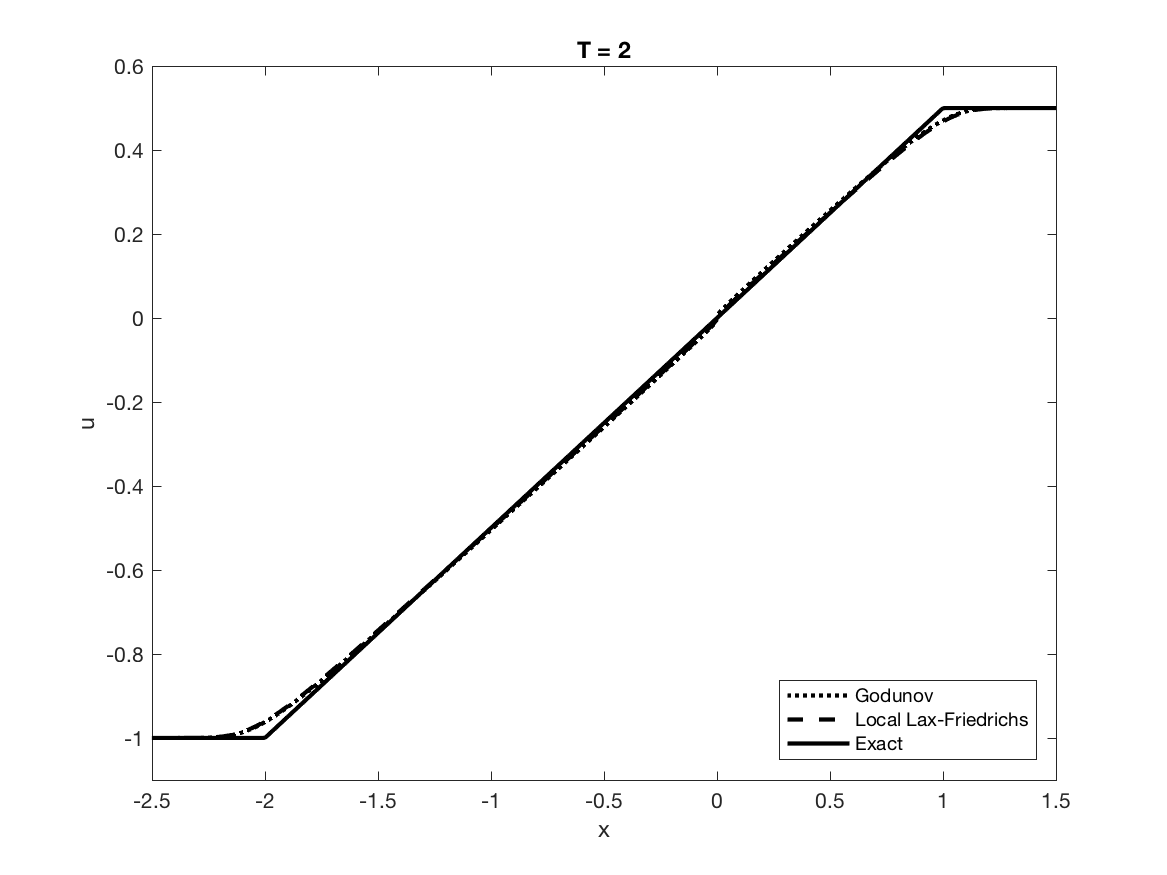
\includegraphics[scale=0.8]{Figures/04_02.png}
    \end{center}

\end{enumerate}
\end{document}
